%*******************************************************************************
%****************************** Second Chapter *********************************
%*******************************************************************************

\chapter{Related Work}
\label{chapter_related}

\ifpdf
    \graphicspath{{Chapter2/Figs/Raster/}{Chapter2/Figs/PDF/}{Chapter2/Figs/}}
\else
    \graphicspath{{Chapter2/Figs/Vector/}{Chapter2/Figs/}}
\fi

This chapter reviews the related work relevant for this thesis. Since there are many different related work areas that all have their relevance to this thesis, this chapter is divided into different sections dealing with each of them in turn. First section \ref{sec_basicDefinitions} introduces and defines basic the basic terminology that will be used in this thesis. Subsequently section \ref{sec_streamMining} gives a broad overview over the general area of mining data streams but lays a focus on the mining patterns as well as prediction algorithms. Section \ref{sec_stock_market_prediction} then provides more details about prediction in the domain of financial data. Finally section \ref{sec_episodes} introduces the concept of episodes and summarizes different episode mining approaches in static databases. TODO: semantic web

\section{Basic Definitions and Terminology}
\label{sec_basicDefinitions}
This section introduces relevant definitions and terminology that was introduced in previous work and will be used in this thesis.

\subsection{Event Processing Terminology}
The basic event terminology in this subsection is paraphrased from the event processing glossary created by the Event Processing Technical Society \cite{luckham2011epts}. Note that some of the definitions may be slightly altered or simplified. This is due to the fact that the event processing technical society uses these terms for a very general description of event processing and event processing architectures and thus some original definitions are more complex than what is needed in this thesis. The definitions given here aim to establish a clear terminology for this thesis.

\begin{mydef}
\textbf{Event} An event is either something that is happening in the real world or in the context of computer science an object that represents a real world event and records its properties. The latter can also be referred to as an event object or an event tuple. Note that the term is overloaded, but the context usually gives a clear indication of what is meant.
\end{mydef}

The event processing society claims that the context usually solves the ambiguity in the above definition. Since this may not always be the case we will only use the term \textit{event} in this thesis to refer to event objects unless it is otherwise specified.

\begin{mydef}
\textbf{Simple Event} A simple event is an event that is not viewed as summarizing, representing, or denoting a set of other events. Sometimes also referred to as a basic events.
\end{mydef}

These two definitions can sometimes cause confusion. It is important to note that the term event is the most general term, since it can refer to any kind of event, be it simple, derived or complex (see definitions \ref{def_derivedEvent} and \ref{def_complexEvent}). A simple event however is the most basic form of an event and often the ingredient for the creation of more complex events:
Given simple events it is possible to derive events from those or the absence of those. For example the absence measurement events of a sensor could be used to derive the event of that very same sensor becoming defect. These events are called derived events:

\begin{mydef}
\label{def_derivedEvent}
\textbf{Derived Event} A derived event or synthesized event is an event that is generated according to some method or based on some reasoning process.
\end{mydef}

It is also possible to combine multiple simple events to form what we refer to as complex events:

\begin{mydef}
\label{def_complexEvent}
\textbf{Complex Event} A complex event is a derived event that is created by combining other events. The events can be combined by using certain operators, for example disjunction, conjunction or sequence. An example would be $(A \land B) \rightarrow C$ (event A and B in any order followed by event C).
\end{mydef}

This is a very broad definition of complex events. The choice of allowed operators strongly impacts the expressiveness of complex events. A specific kind of complex events are episodes (see section \ref{sec_episodes}), which will be the main focus of this thesis.
The next notion that needs to be considered is that each individual event normally belongs to a certain class of events, which we refer to as the event type:

\begin{mydef}
\textbf{Event type} The event type, sometimes also referred to as event class, event definition, or event schema is a label that identifies events as members of an event class.
\end{mydef}

Another important term that was not explicitly defined in the event processing glossary, but is very relevant to the topic at hand is the notion of a type alphabet:

\begin{mydef}
\textbf{Type Alphabet} The type alphabet, often simply called the event alphabet, is the set of all possible event types that can occur in the observed system.
\end{mydef}

Event alphabets are often implicitly defined when mining frequent itemsets, patterns or episodes.
So far we have looked at events without considering the scenario we are most interested in which are event streams. To do so we need the notion of timestamps:

\begin{mydef}
\textbf{Timestamp} A time value of an event indicating its creation or arrival time.
\end{mydef}

Given that we can define an event stream:

\begin{mydef}
\textbf{Event Stream} An event stream is an ordered sequence of events, usually ordered by the event timings.
\end{mydef}

Note that this rather broad definition of an event stream does not assume anything about the kind of event that is contained in it. A stream can contain very basic forms of events (simple events) but can also be made up out of derived events or even complex events. Also other properties for example that the stream is constantly updating (new events coming in) are not considered yet.


\section{Data Stream Mining}
\label{sec_streamMining}
As already mentioned in the introduction data streams present a challenge to data miners in many ways. This section aims to give both a general overview over the broad research area of mining data stream as well as specifically cover the related topics of forecasting and stock market prediction.

 %Section \ref{subsec_patternMining} gives an overview on classical pattern mining and frequent itemset mining approaches. Section \ref{subsec_regression} continues with an outline of the state of the art classification and regression approaches after which section \ref{subsec_prediction} will take a closer look on time series prediction with a focus on financial data and stock market forecasting.
%Section \ref{subsec_dataStreamProcessing} then introduces related work in the very broad research area of processing and mining data streams. Afterwards section \ref{subsec_eventProcessing} presents the research area of general event processing with a focus on the mining of complex events and episodes. Finally section \ref{subsec_semanticWeb} finishes with an overview over the most relevant work (with respect to this thesis) in the research area of the semantic web.

%\subsection{Pattern Mining}
%\label{subsec_patternMining}
%Of all the fields related to this thesis basic pattern mining is arguably the most well researched and widely used related research area. First to mention are of course the standard pattern mining algorithms for frequent itemsets \cite{han2007frequent}. The authors of this paper nicely summarize different approaches, which either use candidate generation and the apriori-principle or pattern growth strategies. Problematic with the original Apriori-Algorithm is of course that while the apriori-principle helps to prune the candidate generation, its runtime can still be exponential. On top of that it requires multiple passes over the database, which is something that can be impossible given large data streams. These general pattern mining algorithms have of course already been modified or improved for more specific purposes. For example event data logs have been used to build predictive models that search for patterns that predict critical events in the log file \cite{chen2014pattern}. \newline
%A rather large subfield of pattern mining is the field of (business) process mining. This particular domain usually evaluates log-files of (business) applications that log sequences of events. These logs can be mined to satisfy many different information needs, for example clustering \cite{vaarandi2015logcluster} or process models \cite{priyadharshini2016analysis}.
%Another approach in the field of business logs and process mining is outlier and anomaly detection \cite{sureka2015kernel}. The authors use the length of the longest common subsequence between event sequences as a distance measure to find unusual patterns of events. This field of interest is especially interesting since there are a lot of business applications, some of which use legacy software, whose behaviour is at times unclear or error-prone. Mining underlying business models or unusual behavior can help identify errors. \newline
%A subfield of pattern mining that is especially relevant for this thesis is sequential pattern mining. Comprehensive overviews are given by Slimani et al. \cite{slimani2013sequential} as well as Zhao at al. \cite{zhao2003sequential}.

\subsection{Data Stream Mining Taxonomy}
\label{subsec_dataStreamMiningTaxonomy}
Many research areas in classical data mining are also of interest when processing streams. As already mentioned in the introduction however, data streams impose severe restrictions on the algorithms, such them having to use only one pass over the data and that they should be incremental. Normally data mining algorithms for the classical scenario in which the underlying data is a static database or even a data-set that fits into main memory have these properties. Thus the algorithms need to be modified and often approximations have to be made. A comprehensive basic overview over the application of different data mining tasks and how they can be applied to streams was comprised by Gaber et. al. \cite{gaber2005mining}. Note that the paper by Gaber et. al. was published in 2005, so quite a lot of work has been done since then, which means that these papers are obviously not present in their literature review. However the overview provided by the authors is still very useful, since it brings structure to the large field of data stream mining. A taxonomy that follows the basic structure of the paper by Gaber et. al. is visualized in figure \ref{fig_streamMiningTaxonomy}.

\begin{figure}[h]
	\centering
  	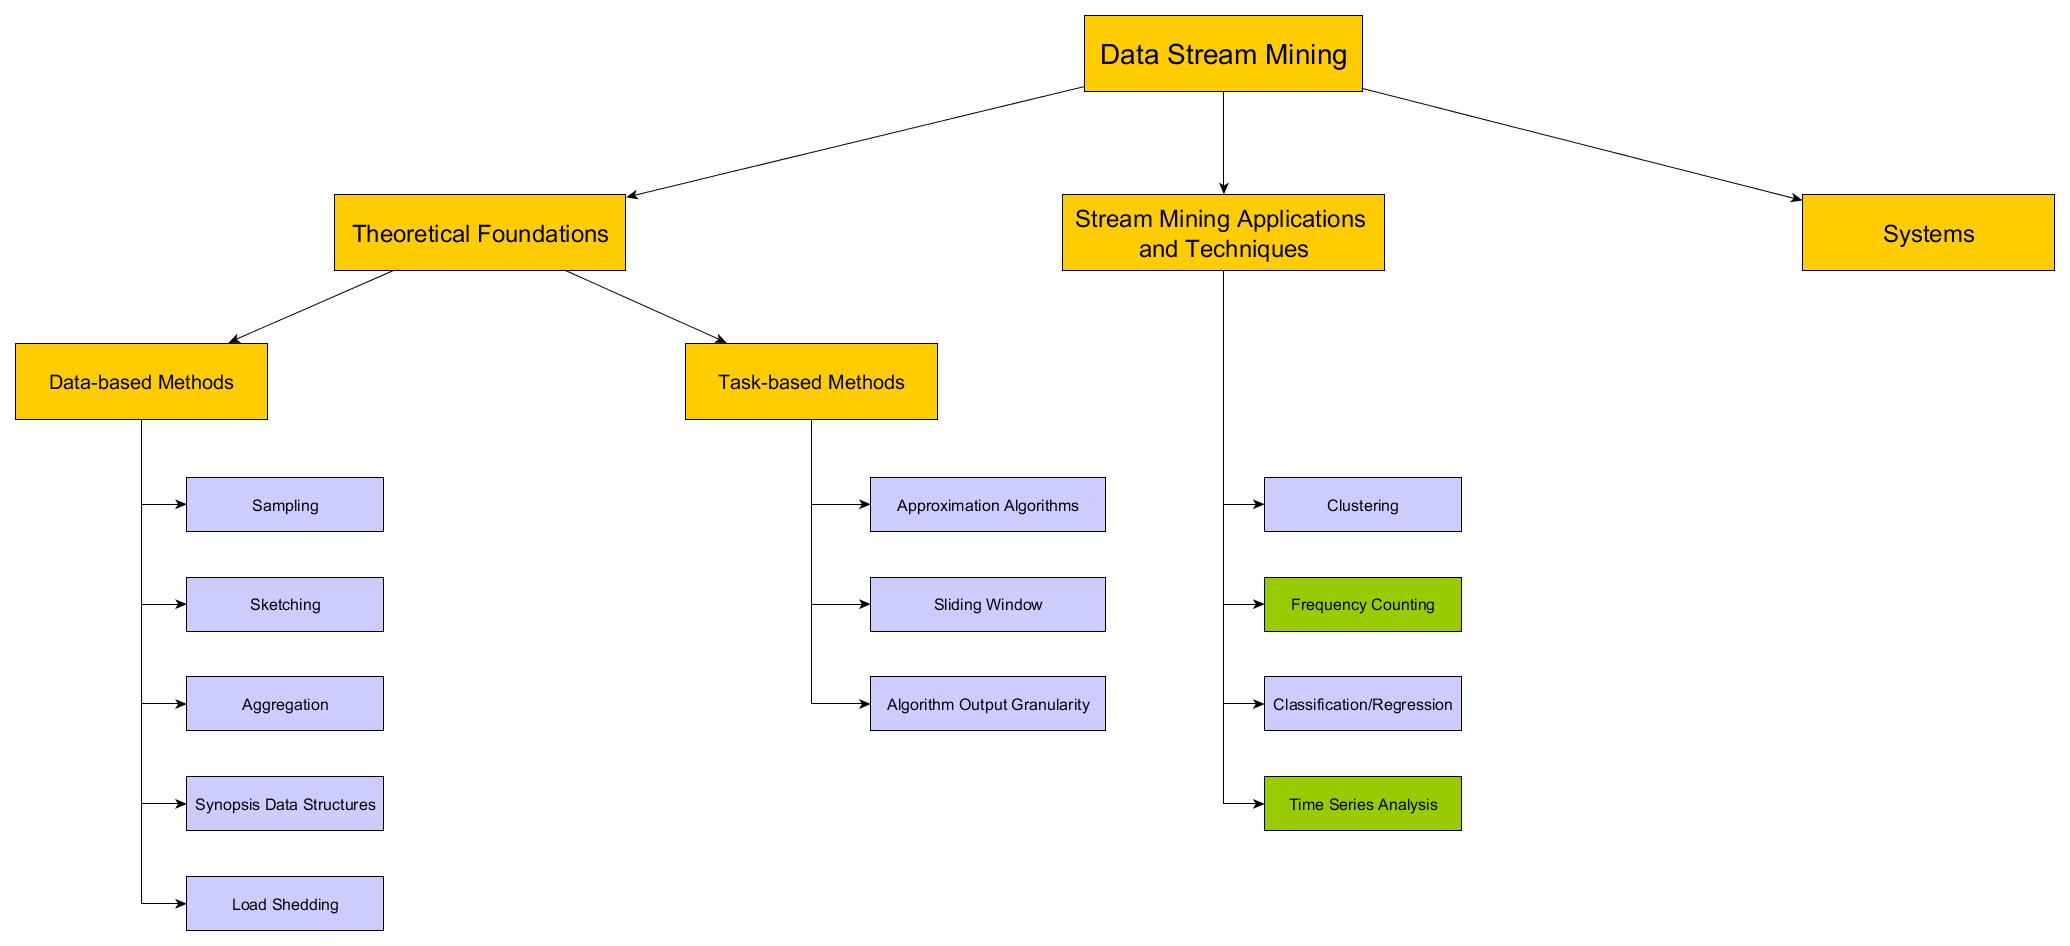
\includegraphics[width=\textwidth]{streamMiningTaxonomy}
	\caption{A taxonomy of the research areas of data stream mining. The subcategories that are marked green are the categories to which this thesis will make contributions.}
	\label{fig_streamMiningTaxonomy}
\end{figure}

As can be seen in the figure the state of the art in data stream mining can be roughly divided into three basic parts:

\begin{enumerate}
	\item Theoretical Foundations
	\item Mining Techniques and Applications
	\item Systems
\end{enumerate}

The theoretical foundations contain general approaches on how to deal with the issues of data streams. There is a distinction between data-based techniques and task-based techniques. Data-based techniques aim to reduce the data being processed or apply transformations on the data stream, while task-based techniques are modifications of existing techniques to meet the requirements for time and space. The subcategories of data-based techniques are:

\begin{itemize}
	\item \textbf{Sampling:} The idea of sampling is basically the same as in statistics. Instead of processing the whole stream, only a subset of the stream is looked at. Due to the unknown size of the stream, sampling methods are more complex than in static systems like databases \cite{manku1999random}. 
	\item \textbf{Load Shedding:} Load shedding is similar to sampling in that it simply drops certain incoming data without processing it, however load shedding is a dynamic approach that is only applied if needed, for example if there are volume spikes (large amounts of data coming in suddenly). Thus in contrast to sampling, which is applied over the whole lifetime of the stream, load shedding is a more reactionary strategy \cite{babcock2003load}.
	\item \textbf{Synopsis Data Structures:} Synopsis data structures summarize the stream in data structures that use less memory than the stream itsself. These data structures are then used to approximately answer queries. A specific subcategory are sketeches, which use very little memory when compared to the whole stream. Examples of this are the so-called frequency moments \cite{babcock2002models}
	\item \textbf{Aggregation:} Aggregation is mainly useful when statistical measures are to be computed over a stream \cite{zhang2002temporal}.
\end{itemize}

The task-based techniques mentioned by the authors are:

\begin{itemize}
	\item \textbf{Approximation Algorithms:} Approximation algorithms are common for hard problems (such as NP-complete problems) but also many classic data-mining problems can be solved on data streams using approximate variants of the original algorithms. A commonly cited example are approxiamtion algorithms for the mining frequent items or itemsets, such as the sticky sampling or the lossy counting algorithm \cite{manku2002approximate}.
	\item \textbf{Sliding Window:} The usage of sliding windows over the data streams is common when the user is only interested in the most recent events as opposed to the complete history. The main challenge here is to construct algorithms that work with the incremental updates that happen whenever new data arrives (the window slides forward). Windows can be defined by either the number of observations in it (sequence-based window definition) or by the duration (timestamp-based window definition) \cite{gama2010knowledge}.
	\item \textbf{Algorithm Output Granularity:} The term algorithm output granularity refers to the strategy of dynamically reacting to the available memory and fluctuating data rates. The basic idea is to mine the incoming data stream as long as possible (normally until the device runs out of memory). If this happens the generated knowledge structures are merged and summarized in order to free up memory and continue the mining. 
\end{itemize}

The second category contains the actual mining techniques and applications, which are well known from classical data mining:

\begin{itemize}
	\item \textbf{Clustering} There are many different approaches that try to apply clustering algorithms to the data stream scenario. Some authors introduce novel methods \cite{aggarwal2003framework} \cite{aggarwal2004framework}, while others modify existing clustering algorithms \cite{guha2000clustering}.
	\item \textbf{Classification and Regression} In Addition to time and memory constraints classification and regression in evolving data streams presents the extra challenges of concept drift, which means that the underlying class distribution may change, which will make the originally built model invalid over time. A commonly used approach to the time and memory constraints are the so-called very fast decision trees \cite{domingos2000mining} which can be built incrementally and require constant time and memory per example.
	\item \textbf{Frequency Counting} Frequency counting is mainly used in conjunction with pattern mining. It is a little unclear why Gaber et. al. decided to name the category frequency counting instead of pattern mining, since all examples that they mention in the frequency counting section of their review count frequencies of items or itemsets, which fit into the category of pattern mining. A reason could be that there exist approaches to counting frequencies that could be generalized to many different pattern mining problems.
	\item \textbf{Pattern Mining} As already mentioned, Gaber et. al. do not explicitly mention pattern mining as a category, however since it is a large field of work and is relevant to this thesis it definately needs to be mentioned. In fact pattern mining in data streams will be looked upon in subsection \ref{subsec_PatternMining} in detail. 
	\item \textbf{Time Series Analysis} Just like pattern mining, time series analysis is especially relevant to this thesis, since predicting (forecasting) future developments based on past data is a large research area in time series analysis. Thus time series analysis in data streams is discussed in detail in subsection \ref{subsec_timeSeriesAnalysis}.
\end{itemize}

The last category in the taxonomy is less focused on research issues and conceptual or algorithmic problems but instead lists the existing data stream processing systems (to that date). Since that is less relevant to this thesis we do not mention or describe existing systems but instead refer the interested reader to the original paper by Gaber et. al. \cite{gaber2005mining}. \\
As visualized in figure \ref{fig_streamMiningTaxonomy} this thesis mainly deals with the subtopics of time series data and pattern mining, which is why these two areas of work will now be inspected more closely in the next subsections

\subsection{Pattern Mining in Data Streams}
\label{subsec_PatternMining}

TODO: is it actually necessary to look at this - the really relevant stuff is done in the episode mining section

\subsection{Time Series Analysis in Data Streams}
\label{subsec_timeSeriesAnalysis}
Before diving deeper into the topic of time series analysis, it is important to distinguish time series from data streams. Both concepts are similar and also have overlapping research areas. In this thesis we speak of a time series if we refer to a temporally ordered sequence of data points, whose time values are sampled at a fixed time interval (QUESTION: is that correct?). Usually time series contain numerical values, examples of such data are:

\begin{itemize}
	\item values of a stock market index over a trading day
	\item measurement values sampled from continous readings of a temperature sensor
	\item electrocardiography readings of a human heart
\end{itemize}

Data streams are also ordered sequences of data. The important distinctions between time series and data streams are: 

\begin{itemize}
	\item Data streams continuously have new data points coming in, thus are continuously growing. This does not have to be the case for time series data. A database that records electrocardiography readings of different patients still contains time series data, however these are not data streams, since the readings are finished and no longer updating.
	\item Data Streams do not have to be sampled at the same time interval, in fact varying time delay between data points is very common here.
	\item In contrast to time series it is common in data streams to have streams of categorical values or events, whereas values of time series are usually numeric.
\end{itemize}

The combination of both, a time series data stream, is a time series that is constantly updating, for example an electrocardiography reading that is currently taking place, or stock values that are being recorded over a day. In these cases the time series must be processed online. \newline
At the first glance this thesis does not seem to be located in the area of time series analysis, since it deals with the mining of complex events. However, since this thesis aims to create a novel method in order to build predictive models using complex events. Predictive models however are commonly build for time series data, since predicting time series (also called forecasting) is of interest in many different domains. Since any novel method needs to be compared to the state of the art it is important to at least give a brief overview, which is what is done here.\\
Most other research areas in data mining such as clustering or classification are rather focussed in their goals (find an appropriate clustering or build an acurate classifier). In contrast to this the research area of time series analysis is more broad, meaning there are a variety of different objectives that can be of interest when analyzing time series. Thus it is helpful to first get an overview over the most common objectives and techniques in a similar way as the taxonomy for data stream mining visualized in figure \ref{fig_streamMiningTaxonomy}. The main source for this subsection is the book by J. Gama \cite{gama2010knowledge}. Figure \ref{fig_timeSeriesInDataStreamsOverview} visualizes the different areas of interest in time series analysis in data streams mentioned by the author.

\begin{figure}[h]
	\centering
  	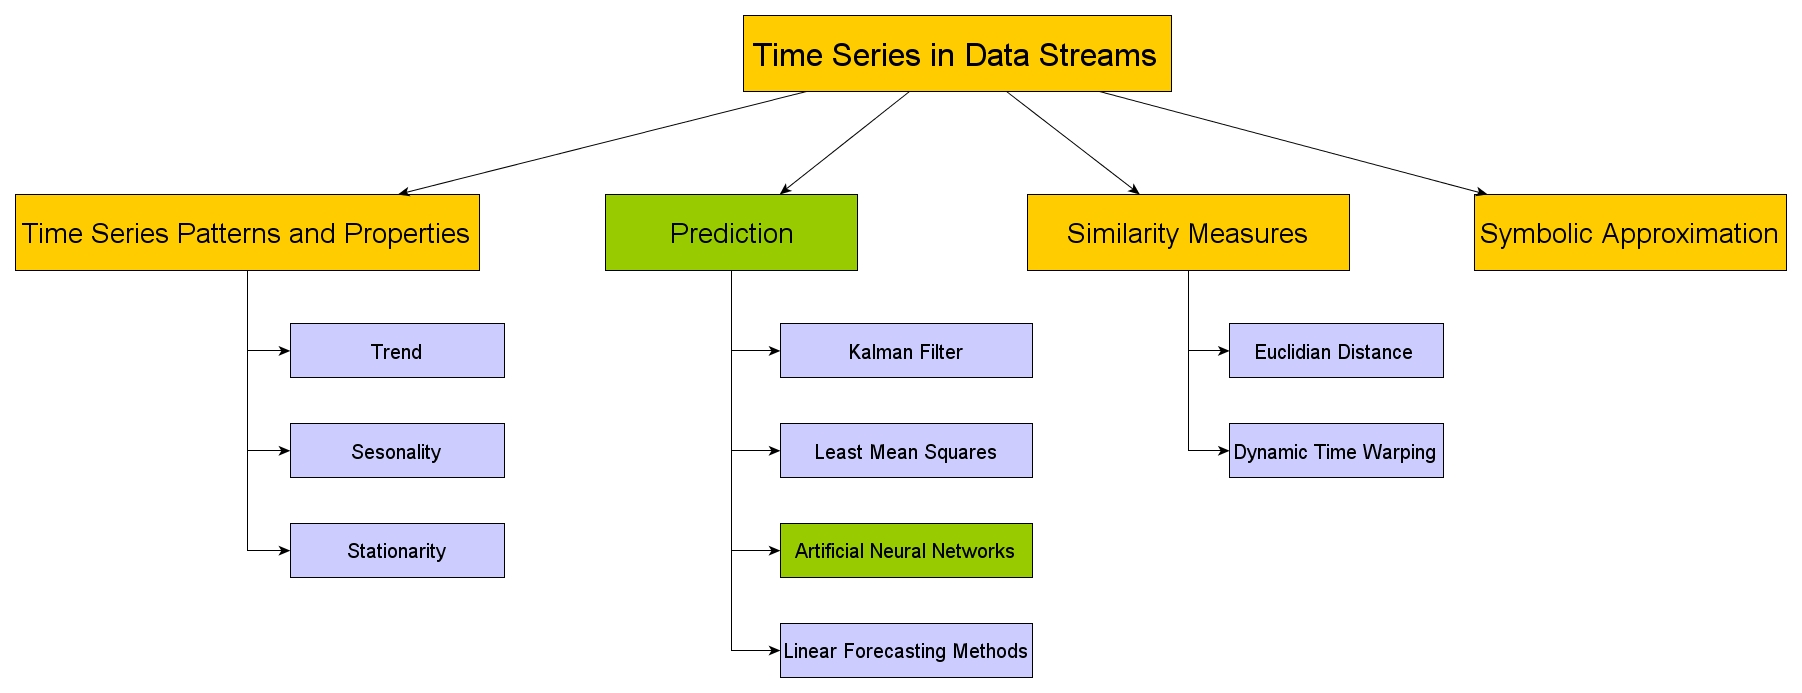
\includegraphics[width=\textwidth]{timeSeriesInDataStreamsOverview}
	\caption{An overview over the different research areas in time series analysis in data streams. The subcategories that are marked green are the categories, which are of interest in thesis and thus will be looked at more closely.}
	\label{fig_timeSeriesInDataStreamsOverview}
\end{figure}

Note that the research area of time series analysis is large and therefore there are important subareas that are not mentioned by the author. Examples of such research areas are curve fitting, function approximation and time series segmentation (QUESTION: Do I need citations for these?). We briefly go over the different areas that are mentioned by J. Game but are not particularly relevant to this thesis:

\begin{itemize}
	\item \textbf{Time Series Patterns and Properties:} A lot of time series can be categorized according to their behavior and can be said to have certain properties. Among these are for example long term trends, seasonality (cyclic behavior) and stationarity ( mean, variance and autocorrelation are constant).
	\item \textbf{Time Series Similarity Measures:} Similarity of time series has many applications and can for example be used in k-NN classification. There are different similarity measures, which each have their advantages and disadvantages. Two well known examples are the classic euclidean distance and the dynamic time warping algorithm.
	\item \textbf{Symbolic Approximation:} Symbolic Approximation is a technique that aims to discretize time series into a string of arbitrary length. It can be of interest if one wants to apply algorithms that work on strings or categorical data to time series.
\end{itemize}

As already mentioned time series prediction (also called forecasting) is relevant for this thesis due to the empirical evaluation which uses financial time series data. Thus, instead of giving a detailed overview over the general topic of time series prediction, we remain rather broad in this subsection and instead we devote the next subsection to exclusively report the state of the art on the prediction of financial time series. \\
Very broadly forecasting methods can be divided into linear and non-linear methods. Linear models are usually simpler, but are at a disadvantage when the underlying model is non-linear \cite{zhang2003time}. Non-linear methods, such as neural networks are more powerful, in fact it has been shown that neural networks can in theory model any non-linear function \cite{abraham2005artificial} \cite{funahashi1989approximate}. However, building and training an actual neural network is a difficult task, since multiple design choices (such as the number of hidden neurons, the activation function and the initial weights) need to be made, which usually requires expert knowledge of both the underlying domain as well as neural networks in general in order to train an appropriate network \cite{abraham2005artificial}. Researchers have also tried to combine both approaches in order to form hybrid methods \cite{zhang2003time}. \newline
Neural networks were originally conceived as batch methods, meaning there were used in an offline scenario with no new data coming in constantly. However adapting them to the stream environment is surprisingly simple in most cases and has been done on multiple occasions \cite{chang2002real} \cite{frank2001time}. In fact, the streaming environment can be beneficial to neural network training, since training a neural network in a static environment usually means making multiple passes over the training data, due to the lack of training data. If done incorrectly this can result in overlearning the training data and thus poor generalization. In the streaming environment however, there is an abundance of data, which means that each example has to be processed only once \cite{gama2010knowledge}. \newline
Predicting or forecasting time series values is normally very domain specific which results in different domains having their own specialized forecasting methods or specific modifications of popular general predictive models. Some of the domains in which time series forecasting is relevant are:

\begin{itemize}
	\item Forecasting price developments in stock markets (see section \ref{sec_stock_market_prediction} for a detailed review of the state of the art)
	\item Forecasting the electricity demands of households \cite{veit2014household}
	\item Forecasting the power output of solar energy plants \cite{inman2013solar}
\end{itemize}

TODO: a few more sentences about forecasting in different domains and why...

QUESTION: maybe explain neural networks ?
%As already mentioned many data mining algorithms for data streams make compromises of some sort or employ appoximations. Especially in the area of pattern mining there are quite a few approaches that use approximations or focus on the most recent data. Gianella et. al. have for example developed an algorithm to incrementally maintain approximately frequent itemsets for the most recent time windows using tilted time window frames \cite{giannella2003mining}. Approaches to mine frequent items without tilting the time windows exist as well, such as the sticky sampling or the lossy counting algorithm \cite{manku2002approximate}. These algorithms can be generalized to mine frequent itemsets, too. If this is done however pruning the candidates may become an issue if the main memory is small (the number of candidates to maintain may be too large). \newline
%A paper also related to regression and time series forecasting was published by Papadimitriou et. al. \cite{papadimitriou2003adaptive}. The authors tackle the problem of cyclic time series mining, as well as time series prediction of numerical values in potentially infinite data streams. \newline
%The rise in popularity of mining data streams also pushes research areas like distributed data mining, in which parallelized versions of data mining algorithms are researched. Large data streams and distributed systems often go hand in hand, which creates the need for distributed algorithms. Such solutions have been researched for example for frequent pattern mining \cite{lin2015fast}, association rule mining \cite{ashrafi2004odam}, clustering \cite{januzaj2004dbdc} and classification (in this case a distributed boosting algorithm) \cite{lazarevic2001distributed}. \newline
%A slightly different direction to data stream processing is querying data streams. Some contributing data scientists have thus approached streams in a similar manner as relational databases \cite{motwani2003query}. The authors present their progress at building a general purpose Data Stream Management System (DSMS) prototype, as a pendant to the traditional Database Management Systems (DBMS). They suggest the usage of an extension of SQL as a stream query language to allow for continuous queries and discuss approximation techniques. 
%
%
%\subsection{Classification and Regression}
%\label{subsec_regression}
%
%Classification and regression are the main applications of supervised learning. They are very similar and closely interlinked to each other. Classification aims to assign new, unseen objects to a class based on a model that was created from training data. Class labels are categorical. Regression is similar, but instead of assigning categorical class labels to new data points it is now the goal to generate a numerical (real) value that is close to the actual value. 
%A comprehensive overview over most classification approaches was comprised by Kotsiantis et. al. \cite{kotsiantis2007supervised}. The authors distinguish between different types of classifiers:
%\begin{itemize}
%	\item logical classifiers such as Decision Trees and rule based algorithms
%	\item preceptron based classifiers, such as the single layered perceptron or artificial neural networks
%	\item statistical classifiers, such as naive bayes or bayesian networks
%	\item instance based classifiers, such as k nearest neighbor
%	\item maximum margin classifiers, such as support vector machines
%\end{itemize}
%It is notable that the authors do not mention ensemble learners \cite{dietterich2000ensemble}, which combine several classifiers and classify new examples by letting each classifier vote. Arguably the most notable ensemble learning technique is the random forest \cite{liaw2002classification}.
%It is important to keep in mind that most classification approaches can also be tweaked to do regression, a random forest for instance can either be used to estimate a (binary) class label (classification) or a numerical value (regression).
%Classification and regression have also been attempted by using pattern mining and association rule generation \cite{ma1998integrating}. Instead of mining all association rules the authors focus on finding so called class association rules. An especially relevant application of rule based regression was the usage of classification rules using minimal rule generation for the prediction of equity returns \cite{apte1994predicting}. The authors modify a classification rule generation technique called R-MINI to be able to do regression. They evaluate their approach on historical stock market data from the S\&P 500 data-set (data is aggregated to monthly values). 
%While both of these pieces of work are interesting and extremely relevant to the problem tackled by this thesis it is important to note that they were both done in 1998 and 1994 respectively, so it is expected that the state of the art has changed since then.



%\subsection{Complex Event Processing and Episode Mining}
%\label{subsec_eventProcessing}
%Before talking about the state of the art in complex event processing it is first important to clarify the term \textit{"event"} which is a is very broad term that is used in many different areas of science. Even when restricted to computer science there may be different definitions with subtle differences. As already explained in the introduction this thesis will focus on events as defined by the glossary of the event processing society \cite{luckham2011epts}.
%When talking about processing complex events there is an important difference between two cases:
%
%\begin{itemize}
%	\item The patterns of interest are known before looking at the data. This is called complex event detection.
%	\item There is no prior knowledge about which patterns might be interesting, they need to be discovered while looking at the data. This is called complex event discovery or complex event mining (which basically means that data mining methods need to be employed)
%\end{itemize}
%
%Complex event detection usually revolves around specification and query languages for complex events \cite{eckert2009complex}. Quite a few different specification and query languages have been developed, such as SNOOP \cite{chakravarthy1994snoop} or the SASE event processing language \cite{wu2006high}. \newline
%Discovering interesting complex events of arbitrary structure in data streams is a very challenging task, thus most work focuses on specific types of complex events. A popular example is mining frequent sequences of events (basically complex events that only use the sequence operator) \cite{bettini1998mining} \cite{hasan2015probabilistic}. \newline
%This thesis deals with a more expressive type of complex events: Episodes. Originally episodes were researched without any relation to event processing \cite{mannila1995discovering}. 
%Episodes have roughly been categorized as serial, parrallel or composite and there are different mining methods proposed for each of these \cite{mannila1995discovering} \cite{zhou2010mining}. The connection between episodes and hidden markov models was also explored in a PHD thesis by Laxman \cite{laxman2006discovering}.
%Evaluating episode mining algorithms on real-life datasets is often difficult due to a lack of knowledge about the ground truth. Thus, generation of realistic, synthetic datasets has been looked into as well \cite{zimmermann2012generating}.



\section{Stock Market Forecasting}
\label{sec_stock_market_prediction}
When reviewing the related work for the forecasting of stock markets, it is important to note that in a lot of cases, financial time series are not analyzed in a streaming environment. Authors commonly attempt to forecast daily closing values of stock markets, which means that in this case data velocity is very low (one new data point per day). However many techniques applied in these scenarios can also be applied in more rapidly moving streams. Examples of these are autoregressive models \cite{terasvirta1994specification} or artificial neural networks \cite{gama2010knowledge}. \newline
A good starting point into the prediction of stock market movements is provided by a literature study by Atsalakis et. al. \cite{atsalakis2009surveying}. The authors review more than 100 papers that attempt to predict stocks or stock indices. Figure \ref{fig_financialTimeSeriesPredictionOverview} visualizes some of the different properties and experimental settings of the approaches covered by Atsalakis et. al.

\begin{figure}[h]
	\centering
  	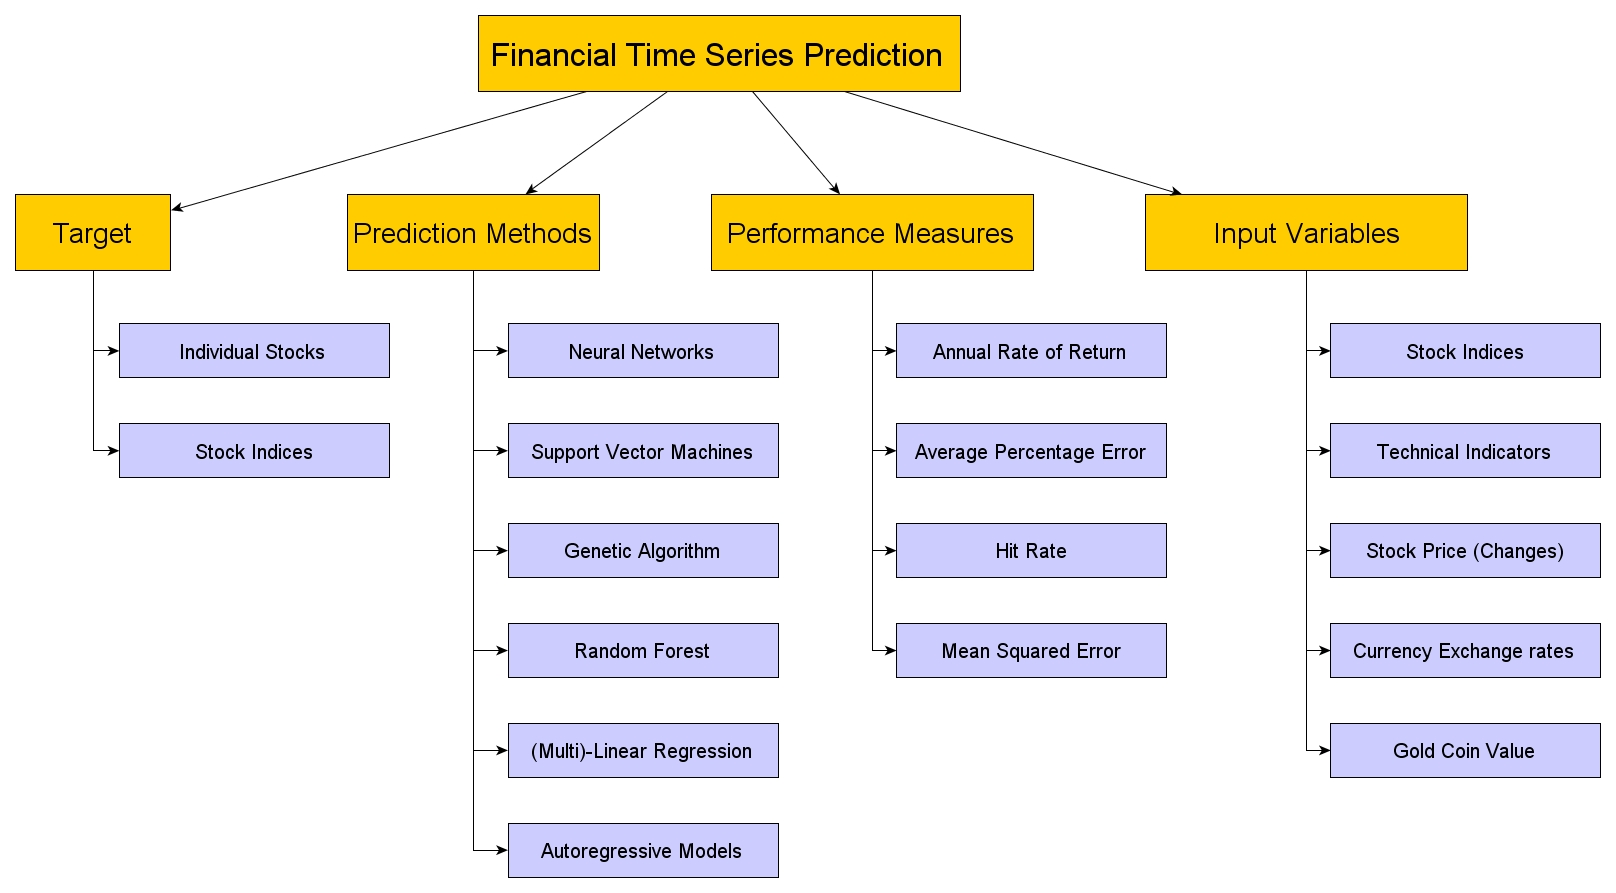
\includegraphics[width=\textwidth]{financialTimeSeriesPredictionOverview}
	\caption{An overview over different properties, experimental settings and approaches to the forecasting of of stock markets}
	\label{fig_financialTimeSeriesPredictionOverview}
\end{figure}

Most of the visualized information in figure \ref{fig_financialTimeSeriesPredictionOverview} was taken from the previously mentioned literature study by Atsalakis et. al. \cite{atsalakis2009surveying}. However  some pieces of work were not covered in that study, for example a comparative study of different models including the otherwise rarely used random forest \cite{kumar2006forecasting}. We briefly review the different properties and categories visualized in figure 
\ref{fig_financialTimeSeriesPredictionOverview}:

\begin{itemize}
	\item \textbf{Target:} The target that is to predict can in theory be any financial index, indicator or price of interst. Many researchers tried to forecast the movement of stock indices \cite{zhang2009stock},\cite{van2001financial}, \cite{kumar2006forecasting} . However, also individual stocks have received attention \cite{mahfoud1996financial}. 
	\item \textbf{Performance Measures:} When building models it is crucial to measure their performance to enable comparison to other models. The number of different performance measures in this case is surprisngly large and diverse. The employed measures range from economic measures, such as the annual rate of return or the Hit-Rate to more technical measures such as the average percentage error or the mean squared error to only name a few. It is impractical to visualize or enumerate all measures that are in use, thus we limit ourselves to the previous examples. For a comprehensive list we refer the reader to the literature study by Atsalakis et. al. \cite{atsalakis2009surveying}.
	\item \textbf{Input Variables:} In real world scenarios this is probably the most important category. No matter which kind of elaborate model is built, if the choice of the input variables is poor, meaning they contain little information, then the model built from those simply can not perform well. This is especially true for financial time series, since those are known to be chaotic and noisy \cite{zhang2009stock}. In fact there are researchers that argue that financial time series follow the principle of random walks which would imply that accurately, meaning better than random, forecasting financial time series based on historical data is impossible. \cite{fama1965behavior}. However there is a considerable amount of papers that suggest otherwise, since accurate prediction results have been achieved by multiple authors based on multiple different forecasting methods (see the literature study by Atsalakis et. al. for examples \cite{atsalakis2009surveying} ). Input variables for stock market prediction are almost always past stock data. Sometimes other financial indicators are used as well. Examples include different stock indices, gold price or currency exchange rates.
	\item \textbf{Prediction Methods:} While figure \ref{fig_financialTimeSeriesPredictionOverview} mentions many different approaches to the forecasting of stock markets, a large majority of the published papers in this area uses some form of neural network. In fact Atsalakis et. al. note that 60\% of the papers they surveyed use feed forward Neural Networks and recurrent networks \cite{atsalakis2009surveying}. 
\end{itemize}

TODO: formulate a nice conclusion


%Similar to regression and classification, but not quite the same is prediction. Prediction (sometimes also called forecasting) introduces a new dimension, which is time. The task in prediction is to build a model that if given data points on a timeline will predict which data point will show up next.
%Due to its dependency on time, prediction plays a large role when mining time series data. Arguably the most popular models for time series prediction are artificial neural networks which are used by multiple authors with differnt variations and application domains \cite{connor1994recurrent} \cite{martinetz1993neural} \cite{frank2001time}. Of particular interest for this thesis are of course prediction approaches that were used in the same domain, namely stock market or financial time series prediction. Naturally this has been looked into. Gestel at. al. used support vector machines to predict the closing values of stock market indices \cite{van2001financial}.% (TODO: Talk/Read more about this paper, the bayesian networks, that are used too) 
%Another, more recent approach used an artificial neural network with an improved learning algorithm (by integrating improved bacterial chemotaxis optimization into the back propagation of the neural network) to successfully predict the Standard’s \& Poor’s 500 index (changes were aggregated to daily values).
%Another different approach is to use grey system models to predict time series \citep{kayacan2010grey}, in this specific case the authors predict the daily foreign currency exchange rate of euro to dollar. A comprehensive comparison of different models for predicting the S\&P CNX NIFTY index was carried out by kumar et. al. \citep{kumar2006forecasting}. The best performing model in their study is the support vector machine, closely followed by a random forest. This is interesting, since random forests have not received as much attention for time series prediction as for example artificial neural networks. Of course no general conclusions can be drawn from the performance of these models for one index. An very detailed overview over a lot of work in the area can be found in the literature study done by Atsalakis et al. \cite{atsalakis2009surveying} although the focus seems to be on papers that use neural networks or support vector machines.
%The attentive reader will have noticed that most of the previously named examples focus on predicting stock indices, a.k.a the general direction of the market. Predicting individual stock values has been looked at less, but there is of source some previous work to be considered. For example mahfoud et. al. compare genetic algorithms to neural networks for the prediction of individual stocks \cite{mahfoud1996financial}.





\section{Episodes}
\label{sec_episodes}
As already mentioned in the introduction, this thesis deals with a specific type of complex events called episodes. Despite being a rather specialized area of research there exists quite a bit of related work that deals with episode mining. What is notable is that there are some discrepancies in terminology. Different authors sometimes use different terms to refer to the same concept or use the same term but with  a different meaning. These discrepancies will be mentioned here and the exact definitions for this paper will be mentioned in chapter \ref{chapter_background}. \\
Before diving into the previous work on episodes it is important to have a rough idea of what kind of patterns episodes are. Thus we provide a short and informal explanation here, whereas section \ref{sec_episodeMiningBackground} will give a much more detailed and formal definition of all concepts revolving around episodes. \\
Most simply put, episode patterns are partially ordered sequences of events. They can be visualized as directed acyclic graphs like the example episode shown in figure \ref{fig_exampleCompositeEpisode}. 

\begin{figure}[h]
	\centering
  	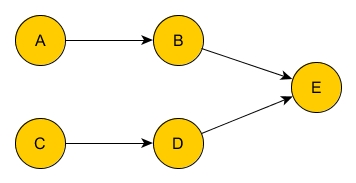
\includegraphics[width=.4\textwidth]{exampleCompositeEpisode}
	\caption{An example episode pattern visualized as a directed acyclic graph. This example pattern specifies that event $A$ and event $C$ may occur in any order, however $A$ must come before $B$ and $C$ must come before $D$, $E$ must occur last.}
	\label{fig_exampleCompositeEpisode}
\end{figure}

Episodes are usually mined from a very large sequence. This distinguishes the concept of episode mining from the concept of sequential pattern mining, which takes place on a sequential database, in which there are many records and each record is a sequence of events \cite{wu2013mining}.
The research concerning episodes can be organized in basic categories as visualized in figure \ref{fig_episodeOverview}.

\begin{figure}[h]
	\centering
  	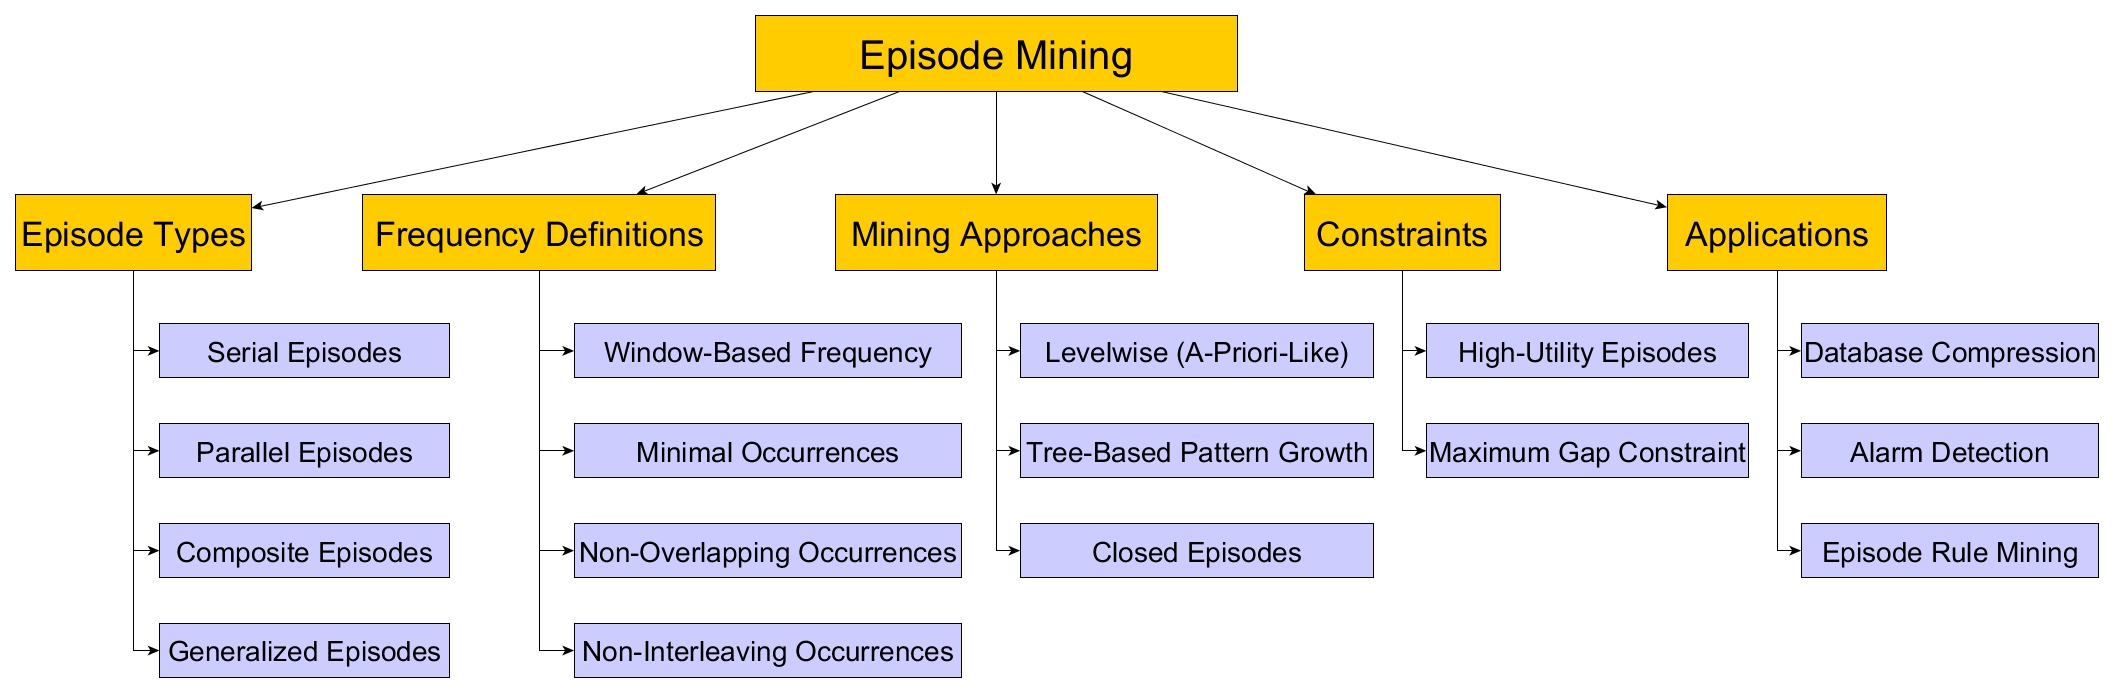
\includegraphics[width=\textwidth]{episodeOverview}
	\caption{A rough categorization of the existing research in episode mining}
	\label{fig_episodeOverview}
\end{figure}

The different types of episodes that have been looked at in the literature are mostly special cases of general episodes. Mannila et. al. introduced the three concepts of serial, parallel and composite episodes \cite{mannila1995discovering}. According to their definitions serial episodes are episodes that have a total ordering (essentially sequences), parallel episodes are episodes without any order (essentially multisets) and composite episodes are episodes that have some order imposed on the events, but do not need to have a total ordering (like serial episodes do). There are however altering definitions of composite episodes in the literature, for example both Bathoorn et. al. \cite{bathoorn2007finding} and Baumgarten et. al. \cite{baumgarten2003tree} deviate from the original definition and redefine composite episodes as sequences of sets. in their works. Section \ref{subsec_basicEpisodeDefinitions} explains the difference between the two definitions in more detail. Extended episodes have been investigated by S. Laxman in his PHD thesis \cite{laxman2006discovering}. The main difference between classic episodes and extended episodes is that classic episodes assume that the basic events are instantaneous, whereas extended episodes can be mined from events that have a duration. It is notable that most work focuses on serial and parallel episodes \cite{mannila1995discovering} \cite{mannila1997discovery} \cite{laxman2006discovering} \cite{laxman2007fast}. Authors have already identified this gap in the research and come up with two different reasons:
\begin{enumerate}
	\item The problem of frequent pattern explosion is already significant for serial and parallel episodes, but still much worse for composite episodes \cite{bathoorn2007finding}.
	\item Detection of composite episodes (checking whether a given composite episode occurs in a sequence) is NP-complete, since 3-SAT can be reduced to this problem \cite{tatti2011mining}.
\end{enumerate}

When mining frequent episodes from sequences, frequency of episodes can be defined in multiple ways. Since the different variants of episode frequency need to be carefully considered in this thesis we do not give a brief overview here but instead devote subsections of chapter \ref{chapter_background} to discuss the different frequency definitions. Specifically subsection \ref{subsec_windowBased} gives a detailed explanation of the window based frequency, whereas subsection \ref{subsec_otherFrequency} provides an overview over the other frequency definitions that have been used in the literature. \\
The different mining approaches for episodes are similar to well known approaches for frequent itemset mining. Since most episode frequency definitions follow the apriori principle, a level-wise approach like in frequent itemset mining \cite{agrawal1993mining} is suggested by many authors \cite{mannila1995discovering} \cite{laxman2006discovering}. As an alternative, tree growth methods have been proposed, in which candidate episodes are represented in a tree data structure that gets grown as the algorithm progresses \cite{baumgarten2003tree}. Since frequent pattern explosion is an issue when mining frequent episodes it is unsurprising that the concept of closed patterns from classical pattern mining \cite{wang2003closet+} has been adapted to episodes \cite{zhou2010mining} \cite{tatti2011mining}. \\
When mining episodes, authors have considered several constraints or specific scenarios. Usually one is interested to mine episodes that are local, meaning the events of the episode are supposed to happen close to each other (time-wise). The maximum duration of an episode can be restrictd in different ways, for example by specifying a window size \cite{mannila1995discovering}, when employing the window-based frequency or by a maximum gap constraint, which restricts the maximum time difference between two events of an episode \cite{meger2004constraint}. Another special scenario that considers external constraints is the mining of high-utility episodes, in which one is not interested in frequent episodes but instead into those episodes that cover events that have a high utility score (which is given externally) \cite{wu2013mining}. \\
The applications for episode mining are diverse and some of them are mentioned in the following.

\begin{itemize}
	\item Mannila et. al. (arguably the researchers to make episode mining a popular task) were motivated to mine episodes in order to analyze alarms in telecommunication systems \cite{mannila1997discovery}.
	\item Several authors attempt to describe, summarize or compress databases or large sequences by mining appropriate episodes. Examples of research in this application area include the work by Bathoorn et. al. \cite{bathoorn2007finding} as well as the work by Vreeken et. al. \cite{vreeken2012summarising}.
	\item Episode mining has been used to extract rules from sequences in several different domains, such as geophysics (finding dependencies between earthquakes) \cite{meger2004constraint} or health care (analysis of temoral dependencies between risk factors for atherosclerosis) \cite{meger2004mining}.
\end{itemize}

\section{Semantic Web}
\label{subsec_semanticWeb}
TODO


%\section*{Subplots}
%I can cite Wall-E (see Fig.~\ref{fig:WallE}) and Minions in despicable me (Fig.~\ref{fig:Minnion}) or I can cite the whole figure as Fig.~\ref{fig:animations}


%\begin{figure}
%  \centering
%  \begin{subfigure}[b]{0.3\textwidth}
%   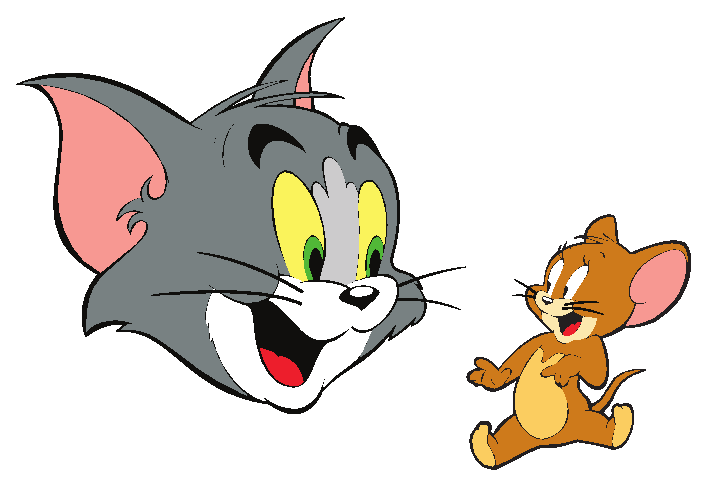
\includegraphics[width=\textwidth]{TomandJerry}
%  \caption{Tom and Jerry}
%    \label{fig:TomJerry}   
%  \end{subfigure}             
%  \begin{subfigure}[b]{0.3\textwidth}
%    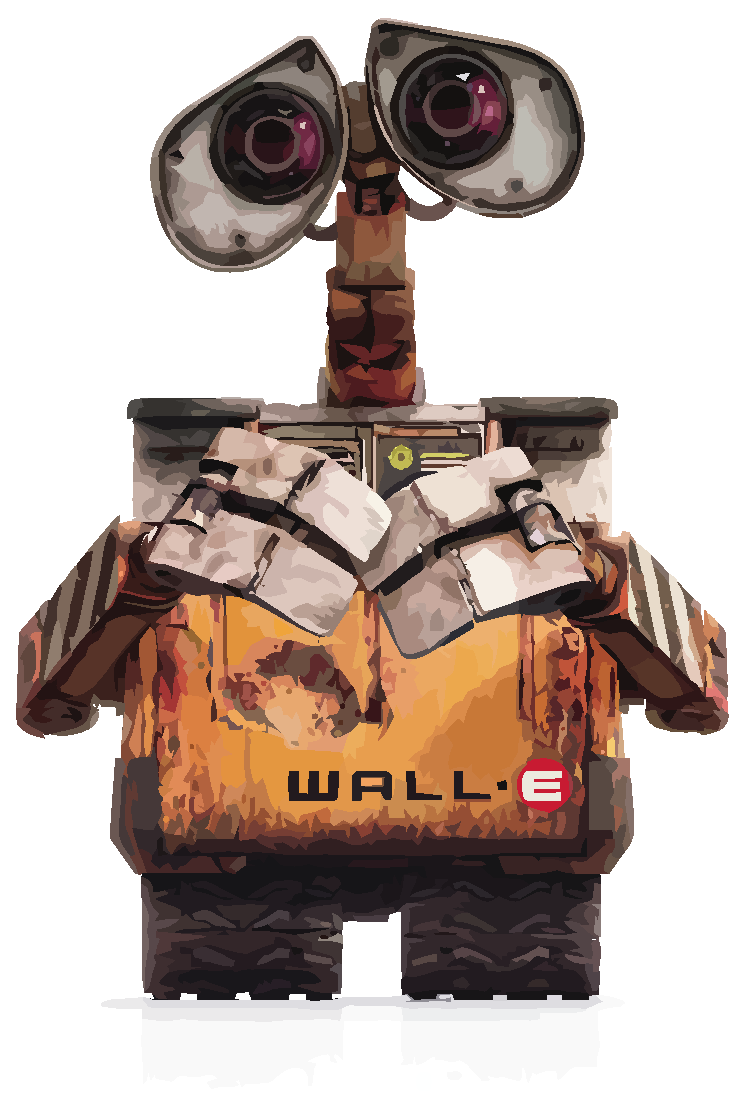
\includegraphics[width=\textwidth]{WallE}
%    \caption{Wall-E}
%    \label{fig:WallE}
%  \end{subfigure}             
%  \begin{subfigure}[b]{0.3\textwidth}
%    
\includegraphics[width=\textwidth]{minion}
%    \caption{Minions}
%    \label{fig:Minnion}
%  \end{subfigure}
%  \caption{Best Animations}
%  \label{fig:animations}
%\end{figure}


